%\documentclass[aspectratio=169]{beamer}
\documentclass[t]{beamer}

\usepackage{./beamer-itmo/beamer-itmo}

\usepackage{graphicx} % support of images
\usepackage{wrapfig} % support of wrapping figures by text
%\usepackage{float} % let you insert images where you really want
\usepackage{mathtext}
\usepackage{braket}
\usepackage{amsmath,amsfonts,amssymb,amsthm,mathtools}
\usepackage{mathrsfs}
\usepackage{icomma}
\usepackage{dsfont} % Badass mathematical font

\usepackage{media9}

\uselanguage{russian}
\languagepath{russian}
\deftranslation[to=russian]{Theorem}{Теорема}
\deftranslation[to=russian]{Definition}{Определение}
\deftranslation[to=russian]{Definitions}{Определения}
\deftranslation[to=russian]{Corollary}{Следствие}
\deftranslation[to=russian]{Fact}{Факт}
\deftranslation[to=russian]{Example}{Пример}
\deftranslation[to=russian]{Examples}{Примеры}
\deftranslation[to=russian]{Figure}{Рисунок}
\deftranslation[to=russian]{Table}{Таблица}

\newcommand*{\heff}{\ensuremath{\mathcal{H}}}
\newcommand*{\Sn}{\ensuremath{\mathbf{S}^{[n]}}}

\graphicspath{{../img/errors/}{../img/}}

% Title

\title[Симплектические методы интегрирования ур-я Ландау-Лифшица]{%
    Симплектические методы интегрирования\linebreak
        уравнения Ландау-Лифшица
}

\author[Плотников Антон]{Плотников Антон Михайлович\linebreak\footnotesize
    Научный руководитель Лобанов И. С.}
\institute{Кафедра высшей математики}
\date{Санкт-Петербург, 2016}

\begin{document}
\ITMOtitlepage

\begin{frame}
    \frametitle{Магнитный скирмион}
    Скирмион -- это квазичастица, представляющая структуру, выстраивающеюся из
    спинов нескольких атомов кристаллической решетки.
    \pause
    \begin{figure}
        \centering
        \includegraphics[width=0.5\linewidth]{skyrmion4}
    \end{figure}
\end{frame}

\begin{frame}
    \frametitle{Уравнение Ландау-Лифшица}
    Состояние магнитной системы описывается уравнением Ландау-Лифшица-Гильберта

    \begin{block}{Уравнение Ландау-Лифшица-Гильберта}
        \begin{equation*}
            \frac{dS_n}{dt} = -\gamma S_n \times \nabla_{S_n} \mathbf E -
            \gamma\lambda S_n \times
            \left(S_n\times \nabla_{S_n} \mathbf E \right)
        \end{equation*}
    \end{block}

    \begin{itemize}
        \only<1>{\item $\mathbf E$ -- энергия системы}
        \item $S_n$ -- вектор направления спина атома с индексом $n$
    \end{itemize}

    \pause

    \begin{block}{Энергия системы}
        \begin{multline*}
            \mathbf E = -\sum_n \Braket{\mathbf B | \Sn} - \mathrm{K_0} \sum_n
            \left| \Braket{\mathbf K | \Sn } \right|^2
            -\\-
            \sum_{n\thicksim m} J^{[n,m]} \Sn - \sum_{n\thicksim m}
            \Braket{\mathbf D^{[n,m]} | \left(\Sn \times \mathbf S^{[m]}\right)}.
        \end{multline*}
    \end{block}
\end{frame}


\begin{frame}
    \frametitle{Метод Эйлера}
    Пусть дана задача Коши
    \begin{block}{Задача Коши}
        \begin{equation*}
            \begin{cases}
                \frac{dy}{dx} = f(x,y) \\
                y_{|x=x_0} = y_0
            \end{cases}
        \end{equation*}
    \end{block}
    тогда следующее значение вычисляется через предыдущее по следующей формуле:
    \begin{block}{Схема Эйлера}
        \begin{equation*}
            y_{i+1} = y_i + hf(x_i, y_i).
        \end{equation*}
    \end{block}
\end{frame}

\begin{frame}
    \frametitle{Неявные методы РК}
    \begin{block}{Неявный метод Рунге-Кутта}
        \only<1>{%
            \begin{gather*}
                S_{n+1} = S_n + h\sum_{j=1}^s b_j f\left(t_n+c_jh, \xi_j\right)
                \\
                \xi_j = y_n + h\sum_{i=1}^{s}a_{ji}f\left(t_n+c_jh,\xi_i\right)
            \end{gather*}
        }%
        \only<2>{%
            \begin{gather*}
                \mathbf S^{[n]}_{k+1} = \mathbf S^{[n]}_k + h\sum_{j=1}^s b_j
                \left[\xi^{[n]}_k \times
                \nabla_{\xi^{[n],k}_j} \mathbf E^k \right]
                \\
                \xi_j^{[n], k} = \mathbf S^{[n]}_k + h\sum_{i=1}^s a_{j,i}
                \left[ -\xi_i^{[n],k} \times \nabla_{\xi^{[n],k}_i}
                \mathbf E^k \right]\label{eq:rk-not-linear}
            \end{gather*}
        }%
    \end{block}

    Коэффициенты $a_{ij}$, $b_i$ и $c_i$ задаются следующей таблицей

    \begin{block}{}
        \begin{figure}[h]
            \renewcommand{\arraystretch}{1.2}
            \centering
            \begin{tabular}{c|ccc}
                $c_1$    & $a_{11}$ & $\ldots$ & $a_{1s}$ \\
                $\vdots$ & $\vdots$ & $\ddots$ & $\vdots$ \\
                $c_s$    & $a_{11}$ & $\ldots$ & $a_{ss}$ \\ \hline
                         & $b_{1}$  & $\ldots$ & $b_{s}$ \\
            \end{tabular}
        \end{figure}
    \end{block}
\end{frame}

\begin{frame}
    \frametitle{Симпелектический метод РК}

    Пусть $M=\left( m_{ij} \right)^s_{i,j=1}$ -- матрица вещественных чисел размера
    $s\times s$, где
    \begin{block}{}
        \begin{equation*}
            m_{ij} = b_i a_{ij} + b_j a_{ji} - b_i b_j,\qquad i,j=1,\dots,s
        \end{equation*}
    \end{block}
    \only<1>{%
        тогда справедлива следующая теорема
    }
    \only<2>{%
        тогда справедливы следующие теоремы
    }
    \begin{theorem}
        Если $M = 0$, тогда метод Рунге-Кутта является симплектическим.
    \end{theorem}
    \only<2>{%
        \begin{theorem}\label{th:quadratic-integrals}
            Симплектический метод Рунге-Кутта сохраняет все инварианты в квадратичной
            форме Гамильтоновой системы.
        \end{theorem}
    }
\end{frame}


\begin{frame}[c]
    \frametitle{Метод Гаусса-Лежандра-Рунге-Кутта}
    \begin{table}[h]
        \renewcommand{\arraystretch}{1.8}
        \centering
        \begin{tabular}{c|cc}
            $\frac12 - \frac{\sqrt3}6$ & $\frac14$                  & $\frac14 - \frac{\sqrt3}6$ \\
            $\frac12 + \frac{\sqrt3}6$ & $\frac14 + \frac{\sqrt3}6$ & $\frac14$ \\ \hline
                                       & $\frac12$                  & $\frac12$
        \end{tabular}
        \caption{коэффициенты для метода Гаусса-Лагранжа-Рунге-Кутта}
    \end{table}
\end{frame}


\begin{frame}
    \frametitle{Гамильтонова система}
    \begin{block}{Система Гамильтона}
        \begin{equation*}
            \begin{cases}
                \dot q_k = \frac{\partial H(p, q)}{\partial p_k}\\
                \dot p_k = -\frac{\partial H(p, q)}{\partial q_k}
            \end{cases}, \qquad k = 1\dots s.
        \end{equation*}
    \end{block}
    \pause
    При наивном численном интегрировании должна появится ошибка с длиной
    вектора $\bar{s}$
    \only<2>{%
        \begin{figure}[h]
            \centering
            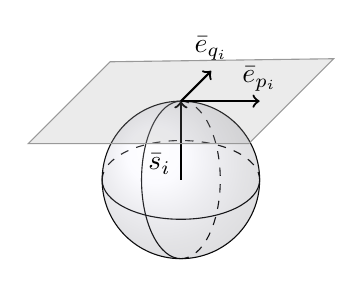
\begin{tikzpicture}
                \draw (-1,0) arc (180:360:1cm and 0.5cm);
                \draw[dashed] (-1,0) arc (180:0:1cm and 0.5cm);
                \draw (0,1) arc (90:270:0.5cm and 1cm);
                \draw[dashed] (0,1) arc (90:-90:0.5cm and 1cm);
                \draw (0,0) circle (1cm);
                \shade[ball color=blue!10!white,opacity=0.20] (0,0) circle (1cm);
            \draw[->, thick] (0,0) -- (0,1) node[left, pos=0.2]{$\bar s_i$};

            \filldraw[black!40, fill=black!40, fill opacity=0.2]
                (-1.4, 1, 1.4) --
                (-1.4, 1, -1.3) --
                (1.4, 1, -1.4) --
                (1.4, 1, 1.4) --
                cycle;

                \draw[->, thick] (0, 1, 0) -- (1, 1, 0) node[above]{$\bar e_{p_i}$};
                \draw[->, thick] (0, 1, 0) -- (0, 1, -1) node[above]{$\bar e_{q_i}$};
            \end{tikzpicture}
        \end{figure}
    }
    \only<3>{%
        \begin{block}{Квадратичный инвариант}
            \begin{equation*}
                L^{[n]} = \Braket{\Sn | \Sn}
            \end{equation*}
        \end{block}
    }
\end{frame}


\begin{frame}
    \frametitle{Метод ньютона}
    Пусть дана система уравнений и начальное приближение $x^0$
    \begin{equation*}\label{eq:newton-needed-form}
        \begin{cases}
            f_1(x_1, x_2,\dots, x_n) = 0\\
            \dots\\
            f_1(x_1, x_2,\dots, x_n) = 0
        \end{cases} \qquad ,
    \end{equation*}
    \pause
    тогда следующее приближение вычисляется как
    \begin{block}{Следующее приближение в методе Ньютона}
        \begin{equation*}\label{eq:newton-generalized-iteration}
            f_i(x^j) + \sum_{k=1}^n \frac{\partial f_i}{\partial x_k}(x^j)
            (x_k^{j+1}-x_k^{j}) = 0,  i=1\dots n \quad .
        \end{equation*}
    \end{block}
    Эту систему можно решить методом би-сопряженных градиентов.
\end{frame}


\begin{frame}
    \frametitle{Тестовый стенд}
    \begin{itemize}
        \item ЦПУ: AMD A8-7100 Radeon R5, 4 ядра, 1800\,МГц
        \item ОС: Arch Linux, x86\_64 Linux 4.5.4-1-ARCH
        \item ЗУПВ:
            \begin{itemize}
                \item SODIMM DDR3 1600\,МГц, 4\,Гб, RMT3170ME68F9F1600
                \item SODIMM DDR3 1600\,МГц, 8\,Гб, CT102464BF160B.M16
            \end{itemize}
        \item \emph{python} 2.7.11
        \item \emph{scipy} 0.17.1
        \item \emph{numpy} 1.11.0
        \item \emph{matplotlib} 1.5.1
    \end{itemize}
\end{frame}

\begin{frame}
    \frametitle{Сравнение ошибки энергии}
    \begin{figure}[h]
        \centernig
        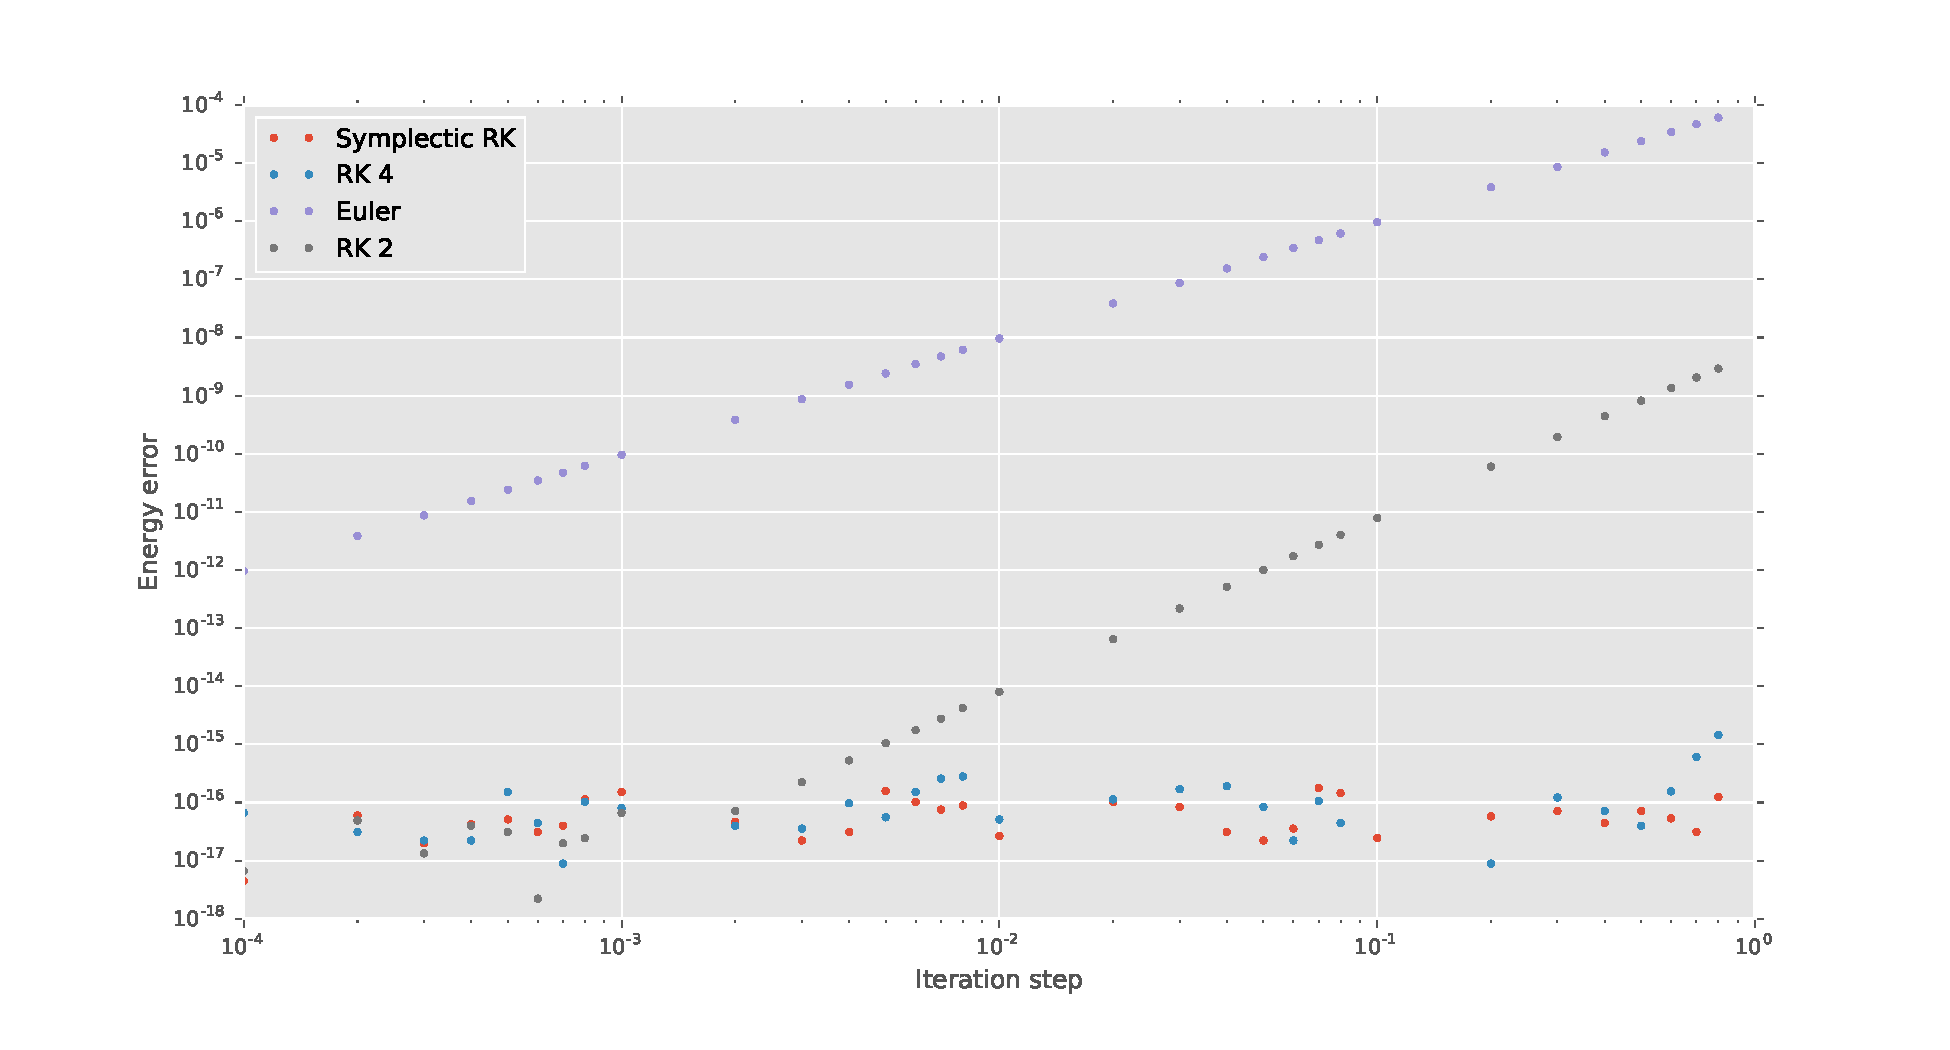
\includegraphics[width=\textwidth]{errorComparsionEnergy}
        \caption{график зависимости ошибки энергии от времени}
    \end{figure}
\end{frame}

\begin{frame}
    \frametitle{Сравнение ошибки длин}
    \begin{figure}[h]
        \centernig
        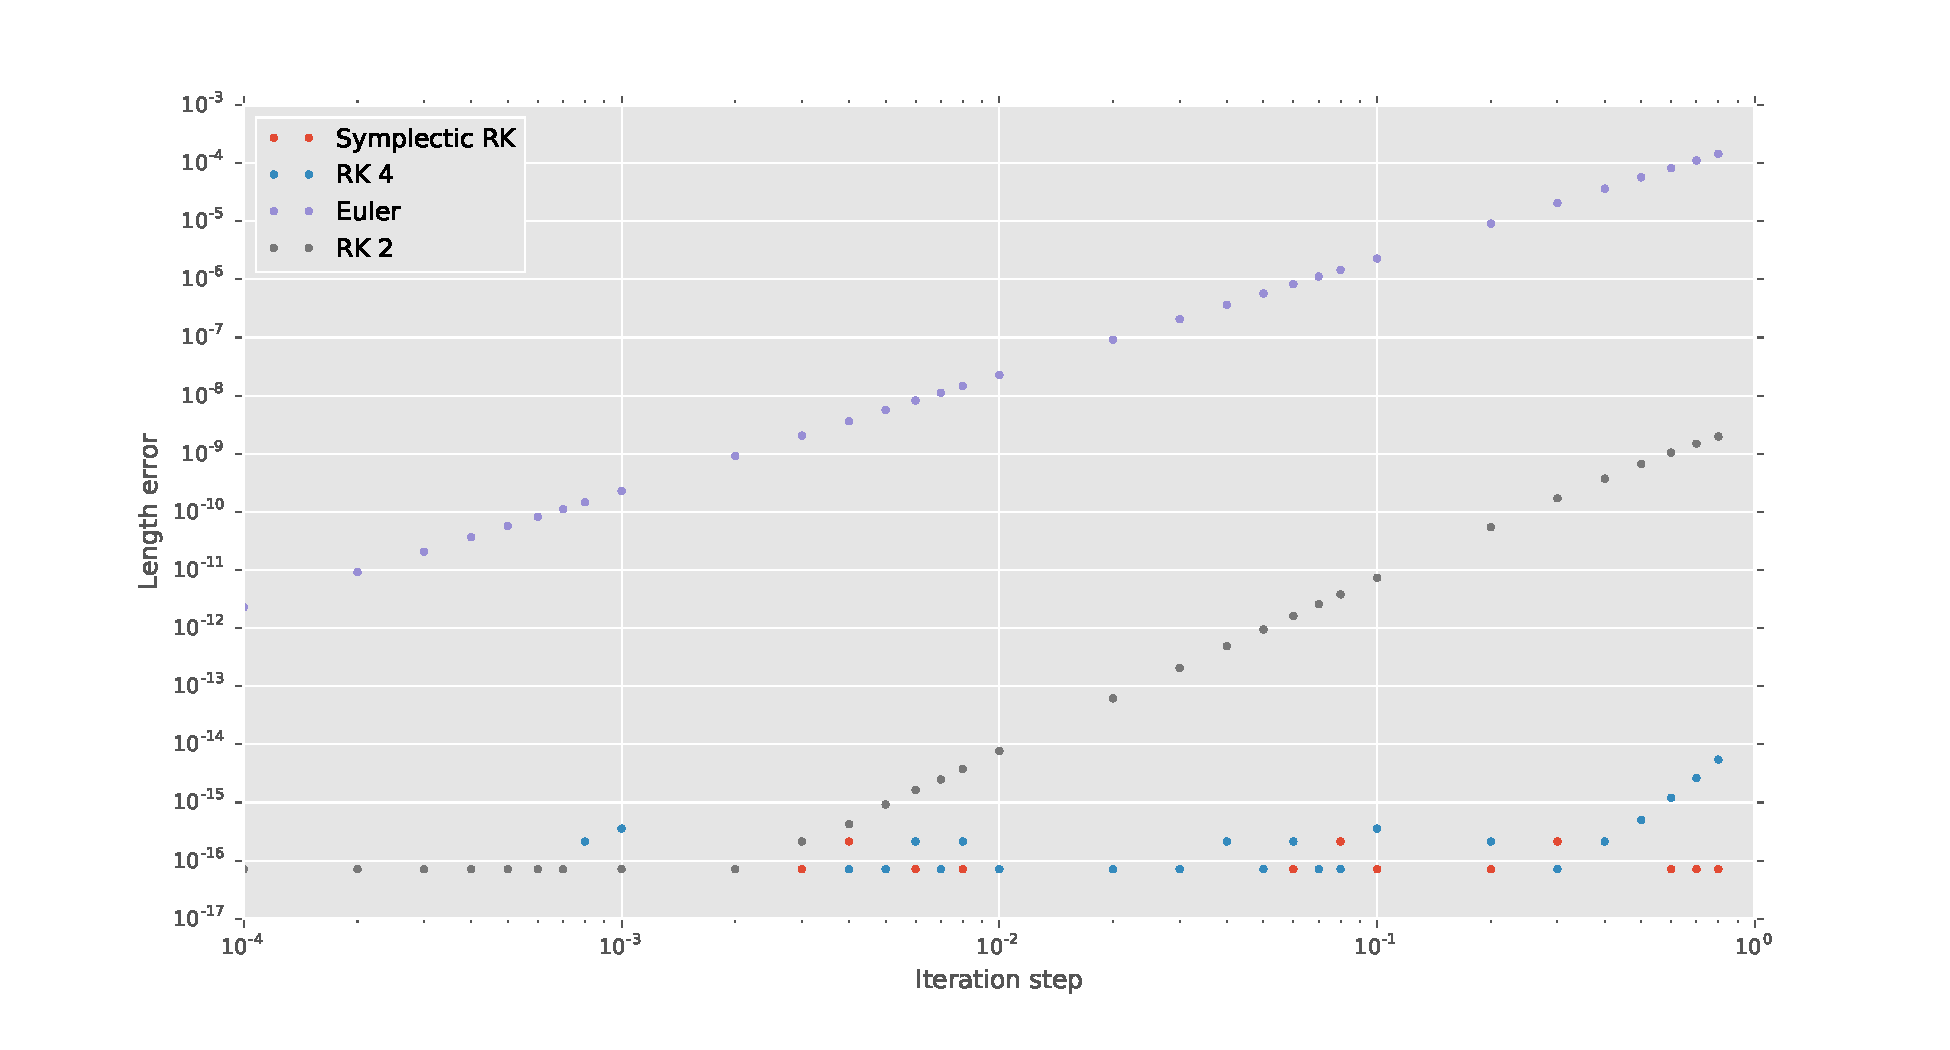
\includegraphics[width=\textwidth]{errorComparsionLength}
        \caption{график зависимости ошибки квадрана суммы длин векторов спинов
        от времени}
    \end{figure}
\end{frame}

\begin{frame}
    \frametitle{Сравнение скорости}
    \begin{figure}[h]
        \centernig
        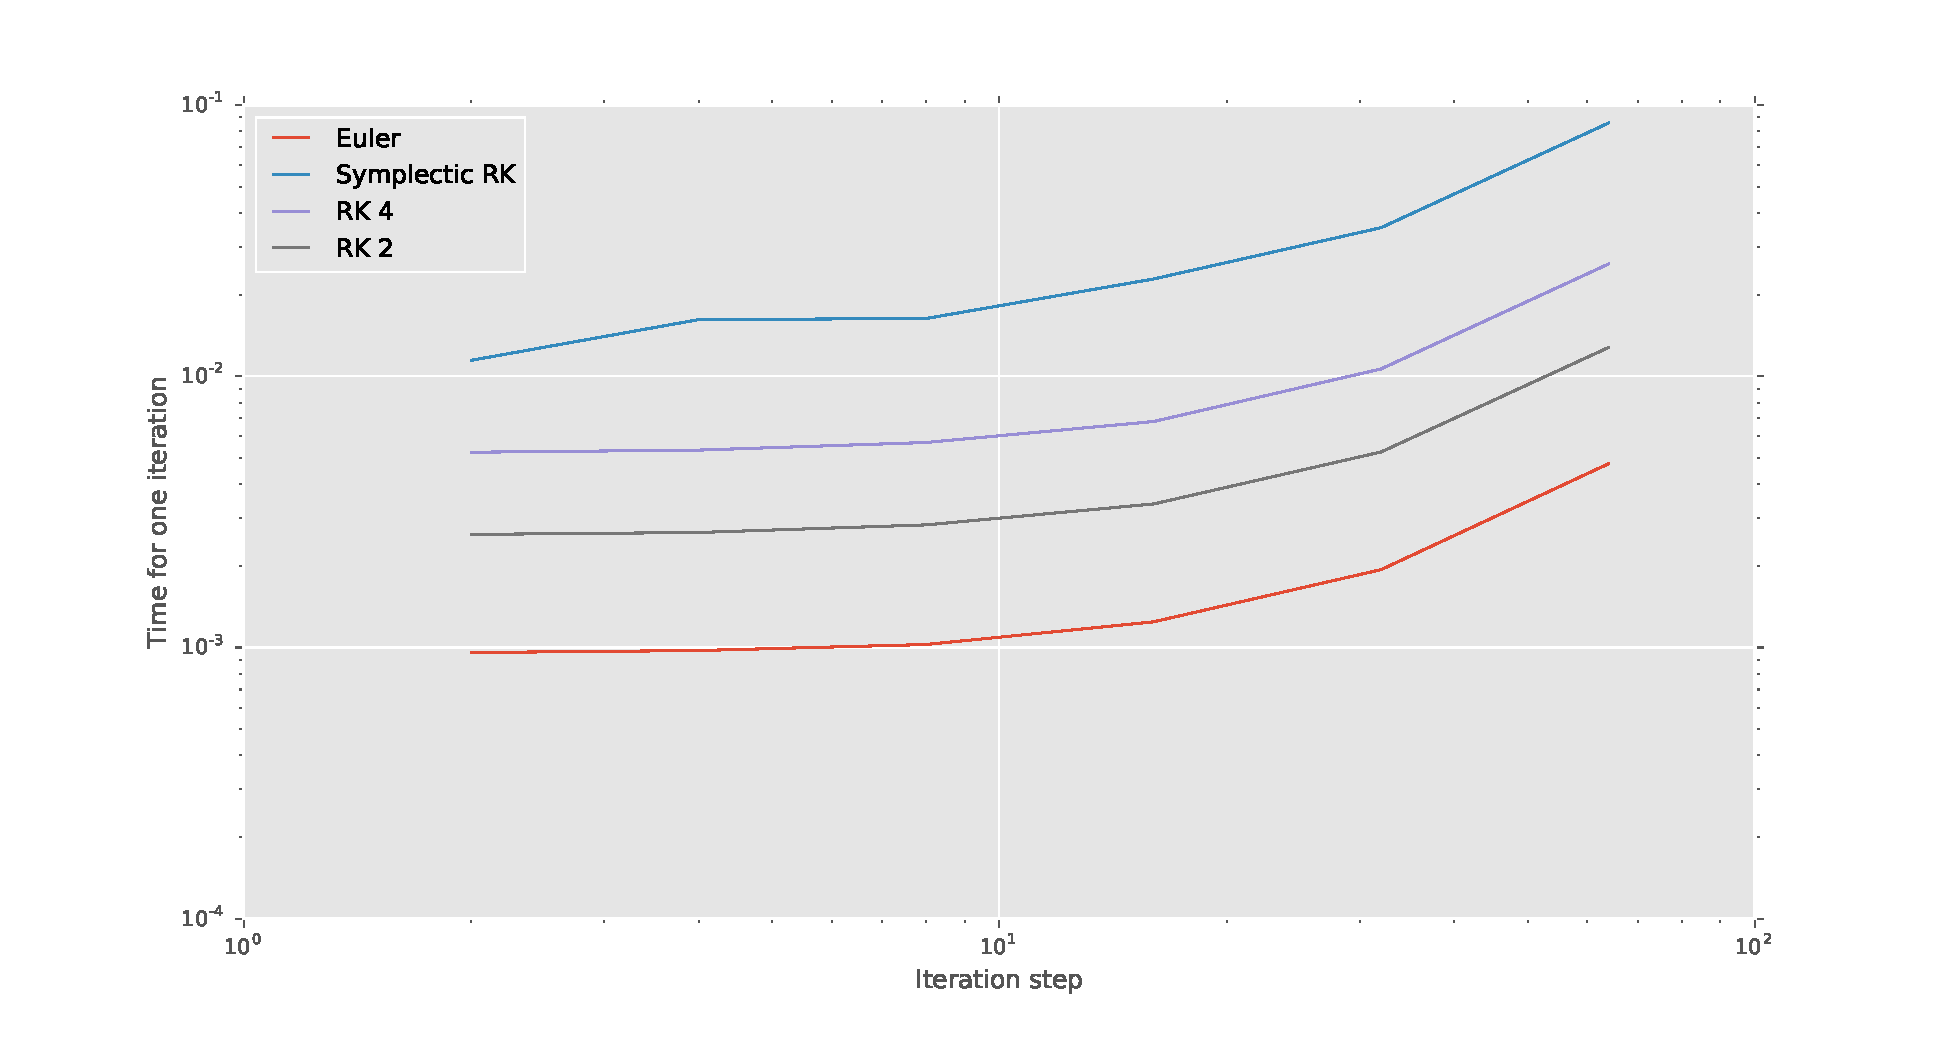
\includegraphics[width=\textwidth]{speedComparsion}
        \caption{график зависимости скорости одной итерации от размера решетки}
    \end{figure}
\end{frame}

\begin{frame}
    %\frametitle{Магнитный скирмион}
	\begin{center}
		\includemedia[
			activate=onclick,
			height=\textheight
		]{\includegraphics{../img/skyrmion4}}{skyrmion.swf}
	\end{center}
\end{frame}

\ITMOthankspage
\end{document}
